% !TEX root = ../team-report.tex
% ERA-Großpraktikum: Team Bericht -- Gruppendynamik

\section{Gruppendynamik}
\label{team:group}

Während \autoref{team:orga} die organisatorischen und technischen Aspekte
der Entwicklung von \erasim{} besprach, ist das Ziel diesen Abschnitts, das
persönliche und menschliche Element zu erörtern. Wir wollen hierbei insbesondere
auf zwei Themen eingehen. Zum ersten möchten wir in \autoref{team:orga-dyno}
die Effektivität unserer Kommunikation sowie die Gruppendynamik des Teams
untersuchen. Zum zweiten wollen wir dann in \autoref{team:orga-conflict} die
aufgetretenen Konfliktsituationen besprechen und analysieren, wie wir diesen als
Team entgegnet sind und welche alternativen Lösungen möglich oder sogar
effektiver gewesen wären als jene, für welche wir uns entschieden.

\subsection{Gruppendynamik und Kommunikation}
\label{team:orga-dyno}

Die wohl wichtigste Säule bei gemeinsamer Arbeit in einem Team, ob für die
Entwicklung eines Assembler-Simulators oder auch jedes sonstige Bestreben, ist
die Kommunikation innerhalb der Gruppe. Insbesondere wird diese Säule
essentiell, wenn sich das Team nicht jeden Tag im Büro begegnet, sondern
verstreut und verteilt, womöglich sogar in verschiedenen Teilen der Welt, am
gemeinsamen Ziel arbeitet. Da die meisten Mitglieder des \erasim{}-Teams
aufgrund des Studentenlebens, wie bereits besprochen, nur unregelmäßig verfügbar
waren, und der Gruppenleiter auch den Großteil des Entwicklungszeitraums in
London Praktika absolvierte, war auch für \erasim{} die Instandhaltung
effektiver Kommunikationskanäle und regelmäßiger, virtueller oder persönlicher,
Treffen von höchster Wichtigkeit. Die folgenden Absätze wollen einen Einblick
geben, auf welche Weise uns diese Instandhaltung via \emph{Slack},
\emph{Hangout}s und auch persönlichen Treffen, gelungen ist.

\subsubsection{Slack}
\label{team:orga-dyno-slack}

Unser wichtigster Kommunikationskanal war die Teamchat-Software \emph{Slack}.
Slack, gewissermaßen ein glorifizierter Instant-Messaging Service, erlaubt
sowohl persönliche, $1:1$ Chats, aber auch die Aufspaltung von Kommunikation in
themenspezifische \emph{Kanäle} (engl. \emph{Channels}). Bei der Entwicklung von
\erasim{} verteilten wir unsere Kommunikation hierbei auf zwei Arten von Kanäle:
\emph{Teamkanäle} und \emph{Topickanäle}.

Teamkanäle waren jene Kanäle, wo jede Untergruppe von \erasim{}, also
\emph{Arch, Core, Parser} und \emph{GUI}, Diskussionen führen konnten, die sich
rein mit den Aspekten der Entwicklung von \erasim{} befassten, die jeder Gruppe
entsprachen. In diesen Chats wurde über den Fortschritt oder aufgetretene
Probleme eines einzelnen Mitglieds der Untergruppe berichtet, wichtige
Informationen zur Entwicklungsumgebung diskutiert (z.B. eine neue Qt Version
oder die Veröffentlichung einer neuen RISC-V Spezifikation) oder auf scheiternde
Tests aufmerksam gemacht. Wichtig hierbei war insbesondere, dass diese Teamchats
nicht für die Untergruppe privat, sondern für das ganze \erasim{} Team
öffentlich war. Somit konnten auch von Mitgliedern anderer Untergruppen Fragen
gestellt bzw. wichtige Entwicklungen mitgeteilt werden. Wollte beispielsweise
ein Mitglied des Core wissen, wie man am besten über die Registergröße der
momentan geladenen Architektur erfährt, so konnte er oder sie diese Frage im
Arch-Chat stellen und ihm oder ihr wurde meist auch schnell geholfen.

Neben Teamkanälen wurde auch kräftig in den Topickanälen diskutiert. Ein
Topickanal beschränkte sich auf ein spezifisches Gebiet der Entwicklung oder
auch anderer Themen. Ein wichtiger und vielgenutzter Kanal war beispielsweise
der C\texttt{++} Channel. In diesem konnten Fragen zu C++ gestellt, stilistische
Aspekte des Google Style Guides diskutiert oder auch bezüglich kryptischen
Kompilierfehlern nachgefragt werden. Mitglieder mit mehr Erfahrung mit der
Entwicklung von C++-Programmen konnten diese Fragen dann beantworten oder auf
entsprechende Ressourcen hinweisen. Ein anderer Topickanal war \emph{report}
genannt, in welchem die Planung und Fertigstellung des ersten und finalen
Berichts besprochen werden konnte. Ein weiteres nützliches Feature von Slack ist
die Integration mit externen Dienstleistungen. So gab es einen weiteren
Topickanal, genannt \emph{notifications}, in welchen wir unseren Test-Server
\emph{Travis CI} integriert hatten. Jedes Mal, wenn unsere Tests auf Travis
erfolgreich waren oder scheiterten, erhielten wir in diesem Kanal eine
Benachrichtigung. Somit musste man auch nicht mehr die Website von Travis CI
besuchen, um über den Status der Tests zu erfahren.

In Summe waren gegen Ende der Entwicklung auf Slack 12 Kanäle offen --- 4
Teamkanäle und 8 Topickanäle. In diesen Kanälen und über private Chats wurde
über den gesamten Entwicklungszeitraum hinweg gesammelt 14,800 Nachrichten
ausgetauscht. \autoref{fig:slack} schlüsselt diese Zahl weiter auf.

\begin{figure}
  \centering
  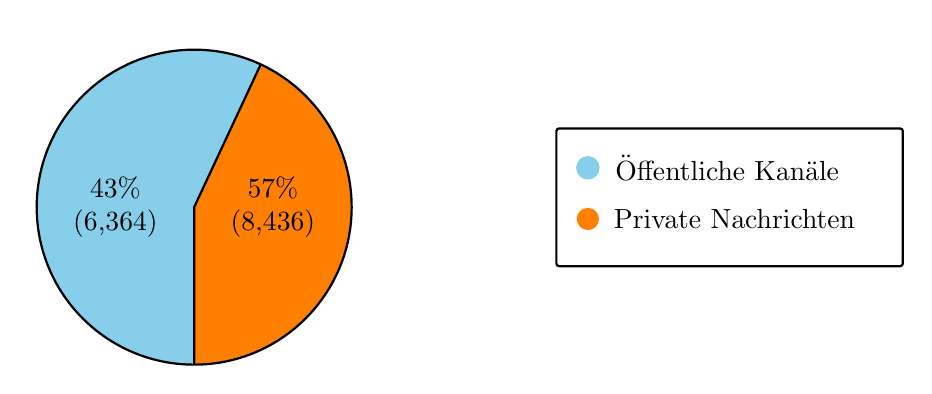
\begin{tikzpicture}[thick]

    % Public Channels
    \fill [SkyBlue]
          (0, -2) -- (0, 0) -- (65:2cm)
          arc [radius=2cm, start angle=65, end angle=270];

    % Direct Messages
    \fill [orange]
          (0, -2) -- (0, 0) -- (65:2cm)
          arc [radius=2cm, start angle=65, end angle=-90];

    % Pie border
    \draw (0, 0) circle [radius=2cm];

    % Sector border
    \draw (0, -2) -- (0, 0) -- (65:2cm);

    % Labels
    \node at (-1, 0) [align=center] { 43\% \\ (6,364)};
    \node at (+1, 0) [align=center] { 57\% \\ (8,436)};

    % Legend
    \path (5, 0.5) coordinate [fill, SkyBlue, circle, inner sep=3pt] (public)
          node [right] {\hspace{0.1cm} Öffentliche Kanäle};
    \fill [orange] (public)+(0, -0.65cm) circle [radius=4pt]
          node [right] {\hspace{0.2cm}\color{black} Private Nachrichten};
    \draw [thick, rounded corners=1pt]
          (public)+(-0.4, +0.5) rectangle ++(4, -1.25);

  \end{tikzpicture}
  \caption{Eine Aufschlüsselung der über Slack versandten
  Nachrichten. Der relative Anteil und die absolute Anzahl an Nachrichten in
  öffentlichen Kanälen sind in Türkis eingezeichnet und private Nachrichten in
  Orange. Insgesamt wurden über 10 Monate hinweg 14,800 Nachrichten verschickt.}
  \label{fig:slack}
\end{figure}

\subsubsection{Hangouts}
\label{team:orga-dyno-slack}

teamchats, topic chats, persoenliche chats
slack

hangouts

persoenliche treffen in der gruppe

was dabei geschah

\subsection{Konfliktsituationen}
\label{team:orga-conflict}
